\documentclass[preprint]{sigplanconf}
\usepackage{xspace,url,subfigure,,framed,
            hyperref, graphicx, fancyvrb % double brackets llbracket
}

\usepackage[T1]{fontenc}
\usepackage{beramono}
\usepackage{listings}
\usepackage{textcomp}
\usepackage[usenames,dvipsnames]{xcolor}
\usepackage{amsmath}

\lstdefinelanguage{Julia}%
  {morekeywords={abstract,break,case,catch,const,continue,do,else,elseif,%
      end,export,false,for,function,immutable,import,importall,if,in,%
      macro,module,otherwise,quote,return,switch,true,try,type,typealias,%
      using,while},%
   sensitive=true,%
   morecomment=[l]\#,%
   morecomment=[n]{\#=}{=\#},%
   morestring=[s]{"}{"},%
   morestring=[m]{'}{'},%
}[keywords,comments,strings]%

\lstset{%\lstinputlisting[language=Octave]{BitXorMatrix.m}
    language         = Julia,
    basicstyle       = \scriptsize\ttfamily,
    keywordstyle     = \bfseries\color{blue},
    stringstyle      = \color{magenta},
    commentstyle     = \color{ForestGreen},
    showstringspaces = false,
    stepnumber=1,
    numbers=left
}

\newcommand{\rn}[1]{#1}
\newcommand{\doi}[1]{doi:~\href{http://dx.doi.org/#1}{\Hurl{#1}}}

\newcommand{\xt}[1]{\texttt{#1}}

\newcommand{\OK}[1]{#1\;\text{OK}}
\newcommand{\abstype}[2]{\xt{abstract}~#1 <: #2}
\newcommand{\oftype}[2]{#1::#2}
\newcommand{\m}[2]{{#1}(#2)}
\newcommand{\contype}[2]{\xt{type}~#1 <: #2}	
\newcommand{\any}{\xt{any}}
\newcommand{\jolt}{\xt{Jolt}}

\newcommand{\exact}[1]{{\llbracket #1 \rrbracket_{\xt{exact}}}}
\newcommand{\usable}[1]{{\llbracket #1 \rrbracket_{\xt{}}}}
\renewcommand{\ldots}{...}
\newcommand{\cnum}[2]{$\text{#1}_#2$}

\usepackage{stmaryrd}
\usepackage{amssymb}
\usepackage{mathpartir}

\conferenceinfo{NOOL '16}{Month d--d, 20yy, City, ST, Country} 
\copyrightyear{20yy}
\copyrightdata{978-1-nnnn-nnnn-n/yy/mm}
\copyrightdoi{nnnnnnn.nnnnnnn}
\begin{document}
\title{Static Typing Without Static Types --- Typing Inheritance from the Bottom Up} 
\authorinfo{Benjamin Chung \and Paley Li \and Jan Vitek}{Northeastern University}{bchung@ccs.neu.edu \and \{pa.li,j.vitek\}@neu.edu} % Annon : Benjamin Chung, Jan Vitek}{Northeastern University}{}
\maketitle
% We should probably have some more introductory/motivational material herezies

\begin{abstract}
Julia is an untyped imperative programming language designed for scientific computing. 
Despite being untyped, Julia provides a rich runtime type system that includes features such as  
inheritance, but lacks mechanisms to ensure compliance with interfaces.
We propose a static type system for a subset of Julia, called \jolt, that rules out functional interface mismatches
with no syntactic alteration to the core of Julia.
\end{abstract}


\section{Introduction}

Traditional statically typed object-oriented languages have a series of
common idioms: single dispatch~\cite{jls}, figuring out which method
to use in which situation, interfaces~\cite{objinter, fj}, to abstract over 
common means of access, and the means to statically
ensure that those interfaces are adhered to with the correct dispatch call.

These practices are perfectly suitable for many contexts,
as is demonstrated by the success of Java~\cite{jls}, C\#~\cite{csls}, and C++~\cite{cppls}, among others.
These features are not universally applicable, however. Languages such as 
Javascript~\cite{ecma} and Lua~\cite{lualang} have no mechanism to define enforced
interfaces, but commonly use documentation-defined interfaces to define behavior
for classes of objects~\cite{lualang}.

\begin{figure}[h]

\lstinputlisting[language=Julia]{broken.jl}
\begin{Verbatim}[fontsize=\scriptsize]
ERROR: MethodError: no method matching a(::C3)
Closest candidates are:
  a(::C1)
  a(::C2)
\end{Verbatim}
\caption{Object inheritance example in Julia.}
\label{code:broken}
\end{figure}


Julia is another such programming language, as it provides multi-method dispatch 
and an interface system that focuses on an abstract struct-like construct. 
Julia was originally designed for the purpose of scientific computation, in the vein of 
R or Matlab\cite{bezan}, containing a number of features designed specifically to support 
numeric computation and other tasks common in scientific programs.


\section{Julia}

From the perspective of object-oriented language design, Julia has several 
interesting features:
\begin{itemize}
\item Julia is \emph{dynamically typed}, and has no mechanism for statically
checking type correctness. However, as illustrated in Figure~\ref{code:broken},
Julia code does have many types.
\item The purpose behind all of these types is \emph{dispatch}. Julia provides 
full multi-method dispatch based on \emph{runtime type tags}. This lets programmers
write code that is highly specified for a specific value. 
\item Despite having types with methods that operate over them, Julia does not 
allow explicit procedural interfaces, a key feature of traditional object 
systems. Julia's interfaces are called \emph{abstract types}, and they define no 
explicit methods, instead, the abstract types rely upon ``a collection of informal interfaces''
\cite{juliadocu} to abstract over implementations. 
\end{itemize}


\begin{figure}
\centering
\vspace{-1em}
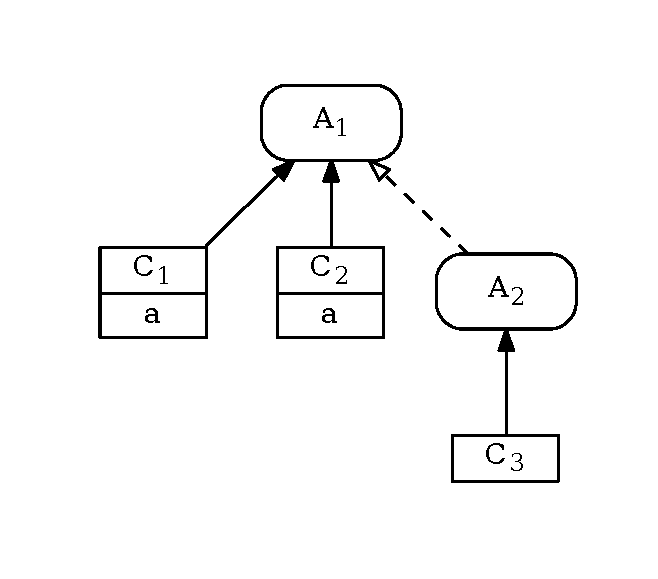
\includegraphics[scale=.6]{example2.pdf}
\vspace{-2em}
\caption{Inheritance hierarchy diagram for Figure~\ref{code:broken}.}
\label{fig:algo}
\vspace{-1.3em}
\end{figure}
Figure~\ref{code:broken} provides an illustration of how these features 
interact, and how they can be used to do untyped object-oriented programming.
The diagram begins by constructing the object hierarchy shown in Figure~
\ref{fig:algo}, as well as a function \texttt{problem}, which calls the function 
\xt{a} on an argument of type $\text{A}_1$.

The next step is to actually call the methods we have defined. Julia performs
dispatch by looking for the \emph{most specific method} whose arguments are
satisfied by the given value - in essence, giving us a type guarantee that the
argument will always be of the declared type. In this way, the implementation 
of \xt{a} on line 7 is called when we call \xt{a} with an instance of $\text{C}_1$
on line 13, and the implementation of \xt{a} on line 8 is called when 
$\text{C}_2$ is passed on line 14.

In this manner, and if we ignore \cnum{C}{3} briefly, the programmer has 
effectively built a functional interface - any \cnum{A}{1} will have an \xt{a} 
method associated with it, and we can use \xt{a} on a \cnum{A}{1} with complete
assurance that it will actually exist. As a result, we have built an interface
by abstracting directly from the concrete implementations.

However, the assumption that \xt{a} is always safe on a \cnum{A}{1} is not true
in this actual program, once we add \cnum{C}{3} back in. Julia does not impose
any constraints on the types in a program, so \cnum{C}{3} is perfectly valid
while lacking \xt{a}. As a result, line 15 produced the listed error, despite 
dispatch having chosen the most applicable method.

This problem is easy to spot in this example, because all of the type definitions
are simple and in the same place. However, in a real Julia program, types can be
imported from other files and exist in much larger hierarchies than the one seen
here. Therefore, a functional interface could be violated by a library, resulting in
errors that are difficult to detect ahead of time.

\section{\jolt}
An interesting observation about the issue identified in Figure~\ref{code:broken}
is that it can be seen as a ``message not understood'' error, exactly the kind
that type systems are widely applied to detect and prevent. However, untyped 
languages are uniquely difficult to type~\cite{cannonpython}, as complex inference is typically
required and the idioms are difficult to track with types.

Other languages, such as Rust, with traits~\cite{rust}, and Haskell, with 
typeclasses~\cite{typeclasses}, have statically checked interfaces for multimethods, but 
cannot handle ``orphan'' implementations - a common idiom in Julia. As a 
consequence, we need to use a new approach.

Despite being untyped, Julia has a considerable
number of types, though they are not used statically. We propose a type system called \jolt\space
for \emph{existing} Julia code that can statically infer interfaces and detect
``method not found'' errors, over a heavily pared down version of Julia.
\jolt\space does not introduce any new types to Julia, instead it uses the existing dynamic
types that already exist in Julia code as static types.
\jolt\space analyses these types statically to detect dynamic errors ahead of time.

\begin{figure}
\begin{align*}f
t ::=~&  C ~|~ s\\
s ::=~& A ~|~ \any\\
d ::=~& \abstype{A}{s} ~|~ \contype{C}{s} \\
  & |~ \m{m}{\oftype{a}{t}, ~\ldots} = e\\
e ::=~& x ~|~ \xt{new} ~ C() ~|~ m(e,~\ldots) \\
\end{align*}
\caption{Static syntax for \jolt.}
\label{fm:syntax}
\end{figure}

\jolt\space formalizes a minimal subset of Julia. In Figure~\ref{fm:syntax}, we present the entire
syntax for \jolt, which consists of types (\xt{t}), declarations (\xt{d}), and expressions (\xt{e}). 
Types in \jolt\space are either a name, which can be the name of an abstract type (\xt{A}) or a concrete type (\xt{C}), 
or the \any\space keyword, which denotes the top type. The declarations 
of \jolt\space consists of declaring an abstract type, declaring a concrete type, and defining the body of a method.
The three expressions in \jolt\space are local variables, object creation, and method invocation. 

Due to the concise nature of this formalism, the expression typing and operational semantics rules for \jolt have
been omitted, as they are straightforward and does not offer much insight into the inheritance structure of Julia. 
Instead, we will focus our attention on highlighting how \jolt\space generates and ensures correctness of the inheritance
hierarchy created from its abstract and concrete types. 

\begin{figure}
\begin{mathpar}
\inferrule*[lab={\tiny TAbsSelf}]{ \m{m}{\ldots, \oftype{a}{A}, \ldots} \in \usable{A}}{ \m{m}{\ldots, \oftype{a}{A}, \ldots} \Subset A}

\inferrule*[lab={\tiny TConSelf}]{ \m{m}{\ldots, \oftype{a}{C}, \ldots} \in \usable{C}}{ \m{m}{\ldots, \oftype{a}{C}, \ldots} \Subset C}

\inferrule*[lab={\tiny TAbsVirtual}]{
	\forall\,C <: A: \m{m}{\ldots, \oftype{a}{C}, \ldots} \in \usable{C}\\ 
	\forall\,A' <: A: \m{m}{\ldots, \oftype{a}{A'}, \ldots} \Subset A'}
{ \m{m}{\ldots,\oftype{a}{A}, \ldots} \Subset A}

\end{mathpar}
\caption{Method enclosure over types.}
\label{fm:methInc}
\end{figure}

In Figure~\ref{fm:methInc}, we present our rules for when methods are enclosed and/or inside a type.
The symbol $\in$ denotes the standard set notion for an element being inside a set. In \jolt,
this means the method is syntactically defined for the type it is in. The symbol $\Subset$ denotes a method being enclosed inside a type. 
In \jolt, a method is enclosed in a type if that method exists in the inheritance hierarchy, but there might not necessarily exist an actual implementation
of that method in the enclosing type. It is important to note the difference between $\Subset$ denoting the semantical relation of methods inside a type that represents its place 
on the inheritance structure, while $\in$ denoting when a method is syntactically defined for a type.

The \textit{TAbsSelf} rule describes when an enclosing method is defined inside that type. 
For concrete types, their enclosing methods are always defined inside themselves, as reflected by the \textit{TConSelf} rule.
The \textit{TAbsVirtual} rule describes the case when an enclosing method in an abstract type 
is not inside that abstract type, which means it's concrete types must have this method inside them
and that all abstract types below this abstract must have this method enclosed within them.

An abstract type is considered correct when three separate components are shown. The first component requires the name of the type to be well-formed, 
the second component requires every method in the type to be well-formed, and the final component requires every method in the type to be enclosed within that type. 
Three similar components are required to show a concrete type is correct.

The key to the implementation of this static type system is computing the 
enclosure relation to satisfy the requirements laid out in Figure~\ref{fm:methInc}.
We propose the straightforward approach, where methods enclosed in an
abstract type $A$ are computed by taking the intersection of all abstract subtypes
$A'$ and concrete subtypes $C$, and combined with the methods that are defined for $A$
itself. 

This bottom-up approach to producing interfaces is the dual of the typical mechanism
for ensuring that classes actually implement their declared interface. In a more
traditional setting, we go from top-to-bottom, checking that the children 
implement a strict superset of the methods on the parent, while our approach 
ensures that the parent has a subset of the methods on the children.

\section{Conclusion}

Julia provides an interesting alternative to traditional functional interface 
definition, whereby the methods of an interface are solely defined by 
the concrete implementations of that interface, instead of having the interface specifying
the methods of its concrete implementation. Despite being
untyped, we are able to utilize this property to create and reason statically about an inheritance
hierarchy within Julia. We demonstrate this approach in \jolt\space, a minimal subset
of Julia. \jolt\space provides static type checking for safe calls of multi-method.

Our approach towards \jolt\space originated from the typed runtime of Julia, which has the potential to
provide the basis for other static analyses. New language features, such as purity, that leverage
existing types in Julia code could also provide additional performance and usability, with few to
no changes required to the existing codebase.

\bibliographystyle{plain}
\bibliography{main}
\end{document}